\title{Midterm 3 for Algebra-Based Physics-1: Mechanics (PHYS135A-01)}
\author{Dr. Jordan Hanson - Whittier College Dept. of Physics and Astronomy}
\date{November 6th, 2017}
\documentclass[10pt]{article}
\usepackage[a4paper, total={18cm, 27cm}]{geometry}
\usepackage{outlines}
\usepackage[sfdefault]{FiraSans}
\usepackage{graphicx}
\usepackage{amsmath}

\begin{document}
\maketitle

\section{Rotational Kinematics}
\begin{enumerate}
\item Suppose the radius of a circular flywheel in a mechanical device is 10 cm.  Recall that the speed of the edge of the flywheel as it rotates is $v = r\omega$, where r is the radius and $\omega$ is the angular velocity.  If the angular velocity is 200 rotations per minute, what is $v$?
\begin{itemize}
\item $\frac{2\pi}{3}$ m/s \textbf{Correct}.  $\omega = \frac{2\pi}{60}(200) = \frac{20\pi}{3}$ radians/sec, so $v = \frac{20\pi}{3(10)} = \frac{2\pi}{3}$ m/s.
\item $\frac{\pi}{2}$ m/s
\item $\frac{3\pi}{2}$ m/s
\item $\frac{4\pi}{5}$ m/s
\end{itemize}
\item Recall that the angular acceleration is $\alpha = \Delta \omega/\Delta t$.  An ice skater begins a spin where the angular velocity is low: 1 rotation per second.  She changes her body position such that she spins at a rate of 6 rotations per second.  If the move takes 2.5 seconds to complete, what is her average angular acceleration?
\begin{itemize}
\item 4 rotations/sec
\item 2 rotations/sec$^2$ \textbf{Correct.} $\Delta\omega/\Delta t = (6-1)/(2.5) = 2$ rotations/second$^2$.
\item 5 rotations/sec$^2$
\item 1 rotations/sec$^2$
\end{itemize}
\item A centrifuge is separating the components of a mixture by spinning the liquid sample at a radius of 5 cm with an angular velocity of 500 rotations per minute.  (a) What is the speed $v$ of the sample?  (b) If the sample is moved to a radius of 10 cm, by what factor will the speed in increase? \\ \\
$v = r\omega$, so $v = 5\times 10^{-2} \left(\frac{2\pi}{60}\right) 500 = \frac{5\pi}{6}$ m/s (2.6 m/s).  If the radius doubles, the speed doubles.  \textbf{This is an example of a scaling problem}.  So the new speed would be $\frac{10\pi}{6} = \frac{5\pi}{3}$ m/s.
\end{enumerate}
\section{Centripetal Acceleration and Centripetal Force}
Recall that the two formulas for centripetal force are: $F_{\rm C} = mv^2/r$, and $F_{\rm C} = mr\omega^2$.
\begin{enumerate}
\item A Formula 1 car with mass 800 kg is racing around a flat turn of radius 100 m.  The static friction coefficient between the car tires and the pavement is 0.1.  Draw a free body diagram that describes the situation. \\
\begin{figure}[ht]
\centering
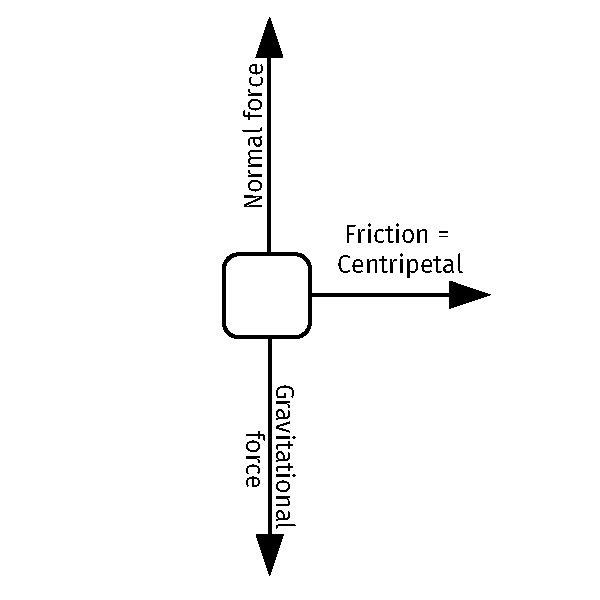
\includegraphics[width=0.2\textwidth]{figures/Friction1.pdf}
\end{figure}
\item Assuming $g = 10$ m/s$^2$, what is the maximum speed with which the car may turn without sliding? \\
$f_C = f_f$, so $mv^2/r = \mu m g$, or $v = \sqrt{\mu rg} = 10$ m/s.
\item Suppose that the car now encounters a banked curve, with a bank angle $\theta$.  Draw a free body diagram that describes the situation (neglecting friction). \\
\begin{figure}
\centering
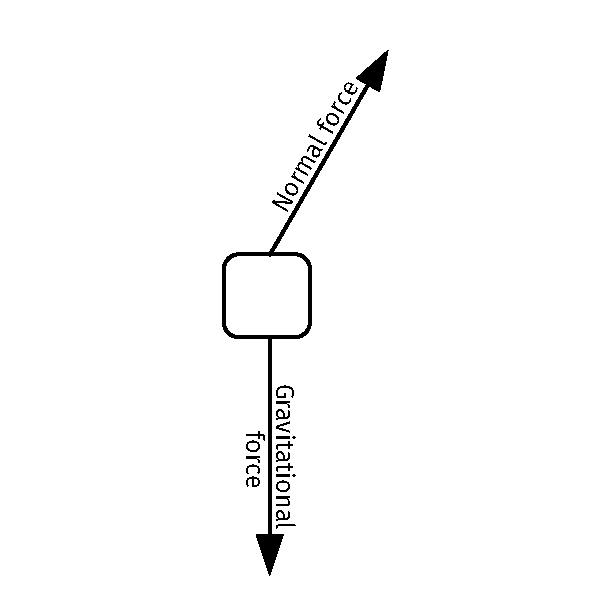
\includegraphics[width=0.2\textwidth]{figures/Bank1.pdf}
\end{figure}
\item By breaking the normal force into two components, show that the bank angle, velocity, and turn radius are related by $\tan\theta = \frac{v^2}{rg}$ (neglecting friction). \\
Let $N$ represent the magnitude of the normal force, $\theta$ the bank angle, $m$ the mass of the vehicle, and $g$ the acceleration due to gravity.
\begin{align}
N\sin\theta &= mv^2/r \\
N\cos\theta &= mg \\
\tan\theta &= v^2/rg
\end{align}
\item If the bank angle is 30 degrees, and the turn radius is 300 m, what is the maximum velocity of the Formula 1 car?  (Let $g = 10$ m/s$^2$). \\
$v = \sqrt{rg\tan\theta} \approx 40$ m/s.
\end{enumerate}
\section{Newton's Law of Gravity, and the Solar System}
\begin{enumerate}
\item Suppose one massive object orbits another.  Which of the following is true about the force of gravity between the objects?
\begin{itemize}
\item The force of gravity on the less massive object by the more massive object is stronger than the force on the more massive object by the less massive object.
\item The force of gravity on the less massive object by the more massive object is weaker than the force on the more massive object by the less massive object.
\item \textbf{The force of gravity on the less massive object by the more massive object is the same as the force on the more massive object by the less massive object.}  This follows from Newton's 3rd Law.  The force depends on both masses, \textit{whether you are talking about the force of one on the other, or vice versa}.
\end{itemize}
\item Apply Newton's Law of Gravity, $F_{\rm G} = G\frac{M m}{r^2}$, and Newton's Second Law, \textit{to show that the acceleration due to gravity at the Earth's surface is 9.8 m/s$^2$}.  $M$ is the mass of the Earth ($6\times 10^{24}$ kg), $r$ is the distance to the center of the Earth ($6000$ km), and $G = 7 \times 10^{-11}$ N m$^2$ kg$^{-2}$. \\
\begin{equation}
mg = \frac{GMm}{r^2} \rightarrow g = \frac{GM}{r^2}
\end{equation}
But putting in the numbers I gave you, which are simplified so you can just do the algebra without calculator (and scientific notation), you get about 11 m/s$^2$.  Well, that's an approximation that becomes 9.8 m/s$^2$ when you make it more accurate.
\item What would the acceleration due to gravity be, if the radius of the Earth was $12000$ km instead of $6000$ km? (Keep all other numbers the same). \\ If we double the radius, the gravitational acceleration should \textbf{decrease by a factor of 4}, because it goes as 1/r$^2$.
\end{enumerate}
\end{document}